\chapter{مفاهیم پایه}

\section{مقدمه}

راه اندازی و استقرار سرویس در صنعت مخابرات به طور سنتی بر این اساس است که اپراتورهای شبکه سخت‌افزارهای اختصاصی فیزیکی و تجهیزات لازم برای هر کارکرد در سرویس را در زیرساخت خود مستقر کنند.
فراهم کردن نیازمندی‌هایی مانند پایداری و کیفیت بالا منجر به اتکای فراهم کنندگان سرویس بر سخت‌افزارهای اختصاصی می‌شود. 
این درحالی است که نیازمندی کاربران به سرویس‌های متنوع و عموما با عمرکوتاه و نرخ بالای ترافیک افزایش یافته است.
بنابراین فراهم کنندگان سرویس‌ها باید مرتبا و به صورت پیوسته تجهیزات فیزیکی جدید را خریده، انبارداری کرده و مستقر کنند.
تمام این عملیات باعث افزایش هزینه های فراهم کنندگان سرویس می‌شود.
با افزایش تجهیزات، پیدا کردن فضای فیزیکی برای استقرار تجهیزات جدید به مرور دشوارتر می‌شود.
علاوه بر این باید افزایش هزینه و تاخیر ناشی از آموزش کارکنان برای کار با تجهیزات جدید را نیز در نظر گرفت.
بدتر این که هر چه نوآوری سرویس‌ها و فناوری شتاب بیشتری می‍گیرد، چرخه عمر سخت‌افزارها کوتاه‍تر می‍شود که مانع از ایجاد نوآوری در سرویس‌های شبکه می‌شود.

در روش سنتی استقرار سرویس شبکه، ترافیک کاربر باید از تعدادی کارکرد شبکه به ترتیب معینی عبور کند تا یک مسیر پردازش ترافیک ایجاد شود.
در حال حاضر این کارکردها به صورت سخت‌افزاری به یکدیگر متصل هستند و ترافیک با استفاده از جداول مسیریابی به سمت آن‌ها هدایت می‌شود.
چالش اصلی این روش در این است که استقرار و تغییر ترتیب کارکردها دشوار است.
به عنوان مثال، به مرور زمان با تغییر شرایط شبکه نیازمند تغییر همبندی و یا مکان کارکردها برای سرویس‌دهی بهتر به کاربران هستیم که نیاز به جا به جایی کارکردها و تغییر جداول مسیریابی دارد.
در روش سنتی این کار سخت و هزینه‌بر است که ممکن است خطاهای بسیاری در آن رخ دهد.
از جنبه دیگر، تغییر سریع سرویس‌های مورد نظر کاربران نیازمند تغییر سریع در ترتیب کارکردها است که در روش فعلی این تغییرات به سختی صورت گیرد.
بنابراین اپراتورهای شبکه نیاز به شبکه های قابل برنامه ریزی و ایجاد زنجیره سرویس کارکردها به صورت پویا پیدا کرده اند.

دو فناوری برای پاسخگویی به این چالش‌ها مطرح شد:

\begin{itemize}
    \item مجازی‌سازی کارکرد شبکه یا \lr{NFV}
    \item زنجیره‌سازی کارکردهای سرویس یا \lr{SFC}
\end{itemize}

با استفاده از مجازی‌سازی کارکردهای شبکه و اجرای آن‌ها بر روی سرورهای استاندارد با توان بالا،
امکان اجرای کارکردها بر روی سخت افزارهای عمومی را فراهم کرده است تا نیاز به تجهیزات سخت افزاری خاص منظوره کاهش یابد.
از طرف دیگر \lr{SFC} امکان تعریف زنجیره کارکردها را ارائه می‌کند که ایجاد
و انتخاب مسیرهای متفاوت برای پردازش ترافیک به صورت پویا و بدون ایجاد تغییر در زیرساخت فیزیکی را امکان‌پذیر می‌کند
با توجه به این فناوری‌ها، مسائل تحقیقاتی جدیدی مطرح شدند که از مهم‌ترین آن‌ها می‌توان تخصیص منابع بهینه به سرویس درخواستی کاربر را نام برد.

از آنجایی که از مفاهیم این فناور‌ی‌ها برای طراحی و تعریف مساله در این رساله استفاده شده است، نیازمند آشنایی با مفاهیم ابتدایی و اصول اولیه آن‌ها خواهیم بود.

بنابراین در این فصل به صورت خلاصه اجزای این فناوری‌ها را مرور خواهیم کرد و کاربردها، چالش‌ها و مسائل تحقیقاتی که در هر یک از این معماری‌ها وجود دارد را مورد بررسی قرار خواهیم داد.

\section{مجازی‌سازی کارکرد شبکه}

مجازی‌سازی کارکرد شبکه اصل جداسازی کارکرد شبکه به وسیله انتزاع سخت‌افزاری مجازی از سخت افزاری است که بر روی آن اجرا می‌شود.
هدف مجازی‌سازی کارکرد شبکه تغییر روش اپراتورهای شبکه در طراحی شبکه
با تکامل مجازی سازی استاندارد فناوری اطلاعات به منظور تجمیع تجهیزات شبکه
در سرورهای استاندارد، سوییچ‌ها و ذخیره‌سازها با توان بالا است.
یک سرور استاندارد با توان بالا سروری است که توسط اجزای استاندارد شده \lr{IT}،
مانند معماری \lr{x86}، ساخته شده و
در تعداد بالایی، مانند میلیون،
فروخته می‌شود.
ویژگی اصلی این سرورها این است که اجزای آن‌ها به راحتی از فروشندگان مختلف قابل خریداری و
تعویض است.
این تجهیزات می‌توانند در مراکز داده، گره‌های شبکه، یا مکان کاربران انتهایی قرار بگیرند.
این روند در
شکل
\ref{fig.6}
نیز توصیف شده است.

\begin{figure}[!h]
\center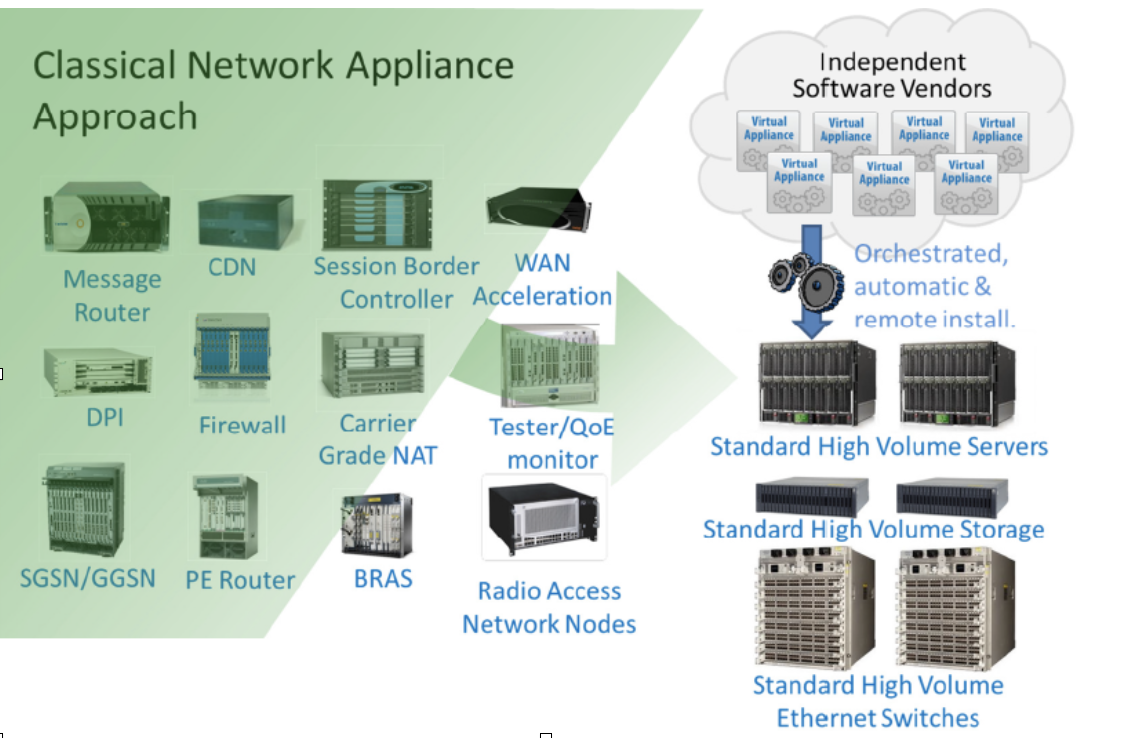
\includegraphics[scale=.5]{images/nfv-concept}
\caption{رویکرد \lr{NFV}}\label{fig.6}
\end{figure}

با استفاده از \lr{NFV}، انواع کارکردهای شبکه مانند دیواره آتش و \lr{NAT}
را می‌توان به صورت یک برنامه نرم‌افزاری از فروشندگان مختلف تهیه کرد و
آن‌ها را بر روی سرورهای با توان بالا اجرا کرد که نیاز به نصب تجهیزات خاص منظوره و
جدید را برطرف می‌سازد.

مزایا و اهداف اساسی که \lr{NFV} برای تحقق و دست‍یابی به آن‍ها شکل گرفته است عبارتند از:

\begin{itemize}
    \item
    کاهش هزینه‌های تجهیزات و مصرف انرژی از طریق تجمیع کارکردها بر روی سرورها و در نتیجه کاهش تعداد تجهیزات
    \item
    کاهش نیاز به آموزش کارکنان، افزایش دسترسی پذیری به سخت افزار و کاهش زمان بازیابی از خرابی سخت افزار به علت استفاده از سخت افزارهای استاندارد و عمومی
    \item
    افزایش سرعت عرضه محصول به بازار با کوتاه‌کردن چرخه نوآوری و تولید. در واقع \lr{NFV} به اپراتورهای شبکه کمک می‍کند تا چرخه بلوغ محصول را به اندازه قابل توجهی کاهش دهند.
    \item
    امکان‍پذیر بودن تعریف سرویس مورد نظر بر اساس نوع مشتری یا محل جغرافیایی. مقیاس سرویس‌ها می‍تواند به سرعت، بر اساس نیاز، گسترش یا کاهش یابد.
    \item
    تشویق به ایجاد نوآوری و ارائه سرویس‌های جدید و دریافت جریان‌های درآمدی تازه با سرعت بالا و ریسک پایین.
    \item
    افزایش توانایی  مقابله با خرابی کارکردها، قابلیت به اشتراک گذاری منابع بین کارکرد ها و پشتیابی از چند مشتری
\end{itemize}

سازمان‌های استانداردگذاری متعددی در استانداردسازی فناوری \lr{NFV} دخیل هستند که شاخص‌ترین آن‌ها موسسه استانداردهای مخابراتي اروپا (\lr{ETSI}) است.
در اواخر سال ۲۰۱۲،
\lr{ETSI NFV ISG}
توسط هفت اپراتور جهانی شبکه به منظور ارتقا ایده مجازی‌سازی کارکرد شبکه تأسیس شد.
\lr{NFV ISG}
تبدیل به یک بستر صنعتی اصلی برای توسعه چارچوب معماری \lr{NFV} و نیازمندی‌های آن شده است و اکنون بیش از ۲۵۰ سازمان با آن همکاری می‌کنند.
اسناد معماری \lr{NFV} به صورت عمومی و رایگان توسط \lr{ETSI NFV ISG} منتشر می‌شود.
ما در این رساله برای توصیف معماری \lr{NFV} از اسناد ارائه شده این سازمان استفاده می‌کنیم.

\section{معماری \lr{NFV}}

در این بخش مؤلفه‌های تشکیل‌دهنده معماری \lr{NFV} شرح داده می‍شوند.
هر یک از اجزای معماری می‍توانند توسط تولیدکنندگان متفاوتی تأمین شوند و به وسیله واسط‌هایی که توسط معماری \lr{NFV}
توصیف شده‌اند با یکدیگر در ارتباط باشند.
بنابراین معماری \lr{NFV} توصیف شده توسط \lr{ETSI} راه‌حلی با قابلیت مشارکت و هماهنگی چندین تولیدکننده مختلف را دارد.
با توجه به استاندارد \lr{ETSI} معماری \lr{NFV}
از سه عنصر کلیدی تشکیل شده است.
زیرساخت مجازی‌سازی کارکردهای شبکه،
کارکردهای مجازی شبکه‌ای و
\lr{NFV MANO}.
این اجزا در شکل \ref{fig.1} نمایش داده شده‌اند.

\begin{figure}[!h]
\center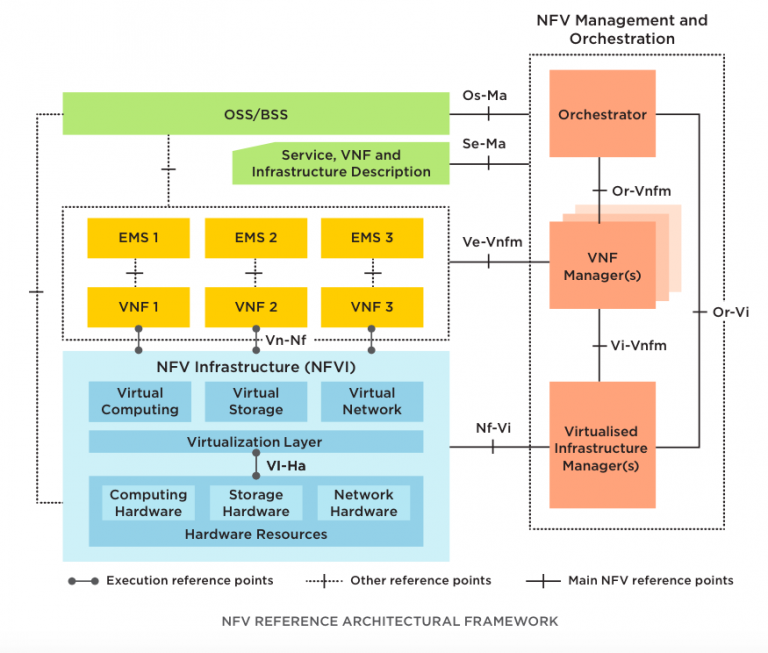
\includegraphics[scale=.5]{images/nfv-arch}
\caption{معماری مجازی‌سازی کارکردهای شبکه
}\label{fig.1}
\end{figure}

\begin{itemize}
    \item
    \lr{NFVI}: شامل منابع سخت افزاری و نرم‌افزاری لازم برای اجرای \lr{VNF}‌ها
    \item
    \lr{Service}: شامل \lr{VNF}‌ها که کارکردهای شبکه را پیاده‌سازی کرده‌اند، \lr{EMS} برای مدیریت \lr{VNF}‌ها و \lr{OSS/BSS} برای ارتباط با سیستم‌های مدیریت سنتی
    \item
    \lr{MANO}: که وظیفه مدیریت و هماهنگی سرویس‌ها و تخصیص منابع را برعهده دارد و از سه بخش \lr{NFVO}، \lr{VIM} و \lr{VNFM} تشکیل شده است.
\end{itemize}

\subsection{زیرساخت مجازی‌سازی کارکردهای شبکه یا \lr{NFVI}}
زیرساخت مجازی‌سازی کارکردهای شبکه ترکیبی از منابع نرم‌افزاری و سخت‌افزاری است
که محیطی برای نصب
کارکردهای مجازی شبکه فراهم می‌آورد.
منابع سخت‌افزاری شامل منابع محاسباتی،
ذخیره‌سازها و شبکه
(شامل لینک‌ها و گره‌ها)
هستند
که پردازش، ذخیره‌سازی و ارتباط را
برای کارکردهای مجازی شبکه فراهم می‌آورند.
منابع مجازی انتزاعی از منابع شبکه‌ای، پردازشی و ذخیر‌ه‌سازی هستند.
به وسیله انتزاع از طریق لایه‌ی مجازی‌سازی (بر پایه‌ی \lr{hypervisor})
منابع سخت افزاری در اختیار کارکردهای مجازی
قرار می‌گیرند که این منابع شامل منابع محاسباتی، شبکه‌ای و ذخیره‌سازی می‌باشند.

در مراکز داده‌ای ممکن است منابع پردازشی و ذخیره‌سازی تحت عنوان یک یا چند
ماشین مجازی نمایش داده شوند در حالی که شبکه‌های مجازی از لینک‌ها و گره‌های مجازی تشکیل می‌شوند.
شبکه‌های مجازی پیش از بحث مجازی‌سازی کارکردهای شبکه مدنظر بوده‌اند و روی آن‌ها کار شده است.
در واقع از شبکه‌های مجازی در مراکز داده‌ای جهت فراهم آوردن شبکه‌های مختلف و مجزا که به کاربران مختلفی تعلق دارند
استفاده شده است. راه‌حل‌های مختلفی برای پیاده‌سازی این شبکه‌ها وجود دارد. در بحث مجازی‌سازی کارکردهای شبکه‌، زیرساخت ارتباطی
مورد نیاز 
برای کارکردهای مجازی از طریق همین شبکه‌های مجازی فراهم آورده می‌شود.
یعنی مسائلی که پیشتر در بحث جایگذاری شبکه‌های مجازی مطرح بود
امروز جزئی از مسائل جایگذاری زنجیره‌های کارکرد سرویس می‌باشند.

\subsection{کارکردهای مجازی شبکه}
یک کارکرد شبکه، یک بلوک عملیاتی در زیرساخت شبکه است که عملکرد رفتاری و رابط‌های ارتباط با خارج خوش تعریف دارد.
مثال‌هایی از کارکردهای شبکه می‌تواند شامل
\lr{DHCP}
یا
\lr{firewall}
و ... باشد.
با این توضیحات کارکرد مجازی شبکه، پیاده‌سازی یک کارکرد شبکه است
که می‌تواند روی منابع مجازی شده اجرا شود.
از هر کارکرد شبکه می‌توان نمونه‌سازی کرده و چند نمونه را در شبکه مستقر ساخت. 
این نمونه‌ها می‌توانند برای سرویس‌دهی به زنجیره‌های مختلف استفاده شوند. از آنجایی که 
هر نمونه توان پردازشی محدودی دارد با افزایش تعداد نمونه‌ها می‌توان توان پردازشی یک کارکرد را نیز افزایش داد.

\subsection{\lr{EM}}
این مولفه کارکردهای \lr{FCAPS} را برای \lr{VNF} ها انجام می دهد که شامل مدیریت خطا، پیکربندی، امنیت، حسابداری و کارایی برای کارکردی است که \lr{VNF} ارائه می دهد. این مولفه ممکن است آگاه از مجازی کارکرد باشد و با همکاری \lr{VNFM} عملکردهای خودش را انجام بدهد.

\subsection{\lr{OSS/BSS}}
این مولفه، ترکیبی از سایر بخش های عملکردهای اپراتور است که در چارچوب معماری \lr{NFV} ارائه شده از طرف \lr{ETSI} قرار نمیگیرند. به عنوان مثال می تواند شامل مدیریت سیستم های \lr{Legacy} باشد.

\subsection{\lr{NFV MANO}}
بر اساس چهارچوب پیشنهادی \lr{ETSI}
وظیفه‌ی \lr{NFV MANO} فراهم آوردن کارکردهای لازم
برای تدارک و فرآیند‌های مشابه مانند تنظیم کردن و ... کارکردهای مجازی شبکه است.
\lr{NFV MANO} شامل هماهنگ کننده و مدیریت کننده چرخه‌ی زندگی
منابع سخت‌افزاری و نرم‌افزاری که مجازی‌سازی زیرساخت را پشتیبانی می‌کنند، است.
هر زنجیره نیاز دارد که حداقل توسط یک \lr{VNFM} مدیریت شود
تا مثلا خطاهای آن را تحت نظر قرار دهد و در صورت نیاز در قسمت دیگری از شبکه استقرار یابد.
مساله‌ی جایگذاری زنجیره‌ها بسیار مورد مطالعه قرار گرفته است، اما در این بین توجه لازم به نیاز این زنجیره‌ها به یک
\lr{VNFM}
صورت نپذیرفته است.

\lr{VNFO} بخشی از مولفه \lr{MANO} است که وظیفه تخصیص منابع به سرویس را برعهده دارد.
یکی از مهم ترین اجزای سرویس گراف \lr{VNF-FG} است که بیانگر \lr{VNF} های سرویس و ارتباطات بین آن‌ها است.
وظیفه اصلی مولفه \lr{NFVO} ایجاد نمونه از سرویس و مدیریت چرخه حیات آن است.
ایجاد نمونه از سرویس شامل ایجاد نمونه از \lr{VNF}‌های تشکیل دهنده آن و ایجاد ارتباط بین نمونه‌ها است.
سایر وظایف مولفه \lr{VNFO} به شرح زیر است:
\begin{itemize}
    \item مدیریت چرخه حیات سرویس شبکه
    \item مدیریت و هماهنگی منابع مورد نیاز \lr{NFVI} بین چندین \lr{VIM}
    \item مدیریت منابع و ایجاد نمونه از \lr{VNF}‌ها با هماهنگی \lr{VNFM}
    \item مدیریت منابع و نمونه‌سازی \lr{VNFM}
    \item مدیریت همبندی نمونه ساخته شده از سرویس شبکه مانند ایجاد، حذف و به روز رسانی \lr{VNF-FG}
    \item مدیریت قالب‌های استقرار سرویس شبکه و \lr{VNF‌}ها مانند اعتبار سنجی قالب‌ها
\end{itemize}
همچنین این مولفه مسئولیت مشخص کردن مکان فیزیکی نمونه های ایجاد شده از \lr{VNF}ها را برعهده دارد.

\section{سرویس شبکه و اجزای آن}
یک سرویس شبکه را می توان به صورت یک گراف جلورانی از کارکردهای شبکه
\lr{(NF-FG)}
که به یکدیگر از طریق زیرساخت شبکه متصل هستند دید.
کارکردهای شبکه می تواند توسط یک یا چند اپراتور ارائه شده باشند.
نقاط انتهایی سرویس را می‌توان به صورت گره‌های گراف و
ارتباطات میان کارکردها را توسط لینک‌های گراف مدل سازی کرد
که لینک‌های گراف می‌توانند، یک طرفه یا دو طرفه، چند پخشی یا همه پخشی باشند.
مثالی از یک سرویس شبکه در شکل
\ref{fig.18}
نمایش داده شده است.
در این شکل، یک سرویس شبکه انتها به انتها از طریق نقاط انتهایی \lr{A} و \lr{B} ایجاد شده که شامل یک \lr{NF-FG} داخلی است.
این \lr{NF-FG} خود شامل سه کارکرد شبکه است که به یکدیگر متصل هستند.


\begin{figure}[h!]
\center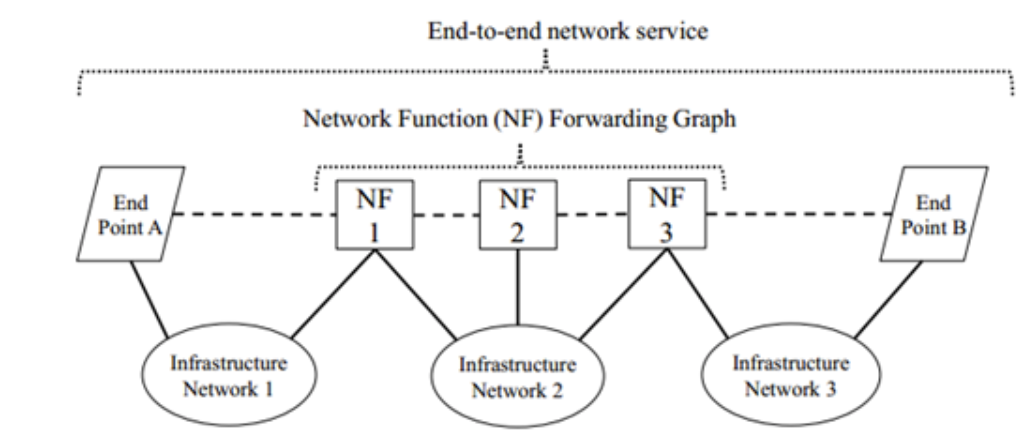
\includegraphics[scale=.5]{images/network-service}
\caption{یک سرویس شبکه شامل یک گراف جلورانی}
\label{fig.18}
\end{figure}

در صورتی که در یک  \lr{NF-FG} حداقل یکی از این کارکردها \lr{VNF} باشد، به آن \lr{VNF-FG} گفته می شود.
در صورتی که فرض کنیم همه \lr{NF} های شکل
\ref{fig.18}
، \lr{VNF} هستند می‌توان آن را مطابق شکل
\ref{fig.19}
نمایش داد.
در این شکل \lr{NF2} خود توسط سه \lr{VNF} پیاده سازی شده است.

\begin{figure}[h!]
\center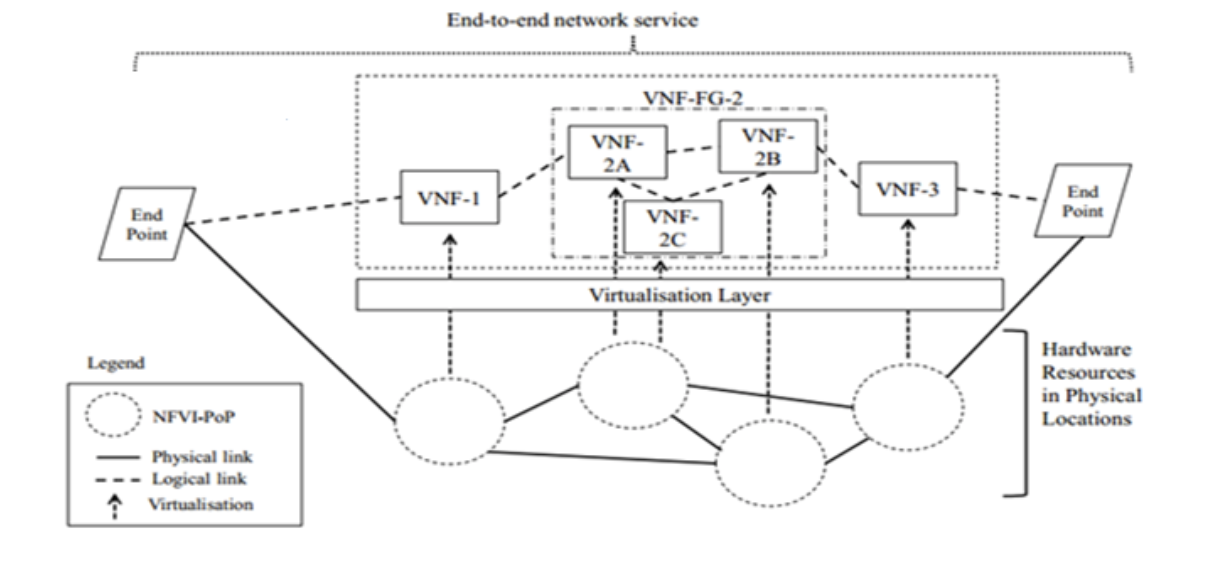
\includegraphics[scale=.5]{images/vnf-fg}
\caption{گراف \lr{VNF-FG} متناظر با شکل \ref{fig.18}}
\label{fig.19}
\end{figure}

مشخص است که گراف \lr{VNF-FG} صرفا ارتباطات بین \lr{VNF}‌ها رو مشخص میکند ولی ترتیب عبور ترافیک از کارکردها را بیان نمیکند.
ترتیب عبور ترافیک از کارکردها توسط \lr{NFP} بیان می‌شود که یکی از اجزای \lr{VNF-FG} است و هر \lr{VNF-FG} باید حداقل یک \lr{NFP} داشته باشد.

\section{موارد کاربرد}
در این بخش موارد کاربرد مهم معماری \lr{NFV} را شرح می دهیم.
یکی از مهم ترین موارد کاربرد ذکر شده برای \lr{NFV} مجازی سازی تجهیزات \lr{CPE} است.
عموما تجهیزاتی در مکان کاربران برای اتصال به اینترنت نگهداری می‌شود که شامل دیواره آتش، \lr{NAT}، مسیریاب و سوییچ است.
در این حالت تنظیمات تجهیزات باید در مکان کاربر صورت بگیرد که هزینه بالایی دارد.
با استفاده از مجازی‌سازی این کارکردها و نگه‌داری آن در سمت \lr{ISP}، میتوان هزینه تجهیزات و زمان نگهداری را کاهش داد.
این مورد کاربرد در شکل \ref{fig.20} نمایش داده شده است.

\begin{figure}[h!]
\center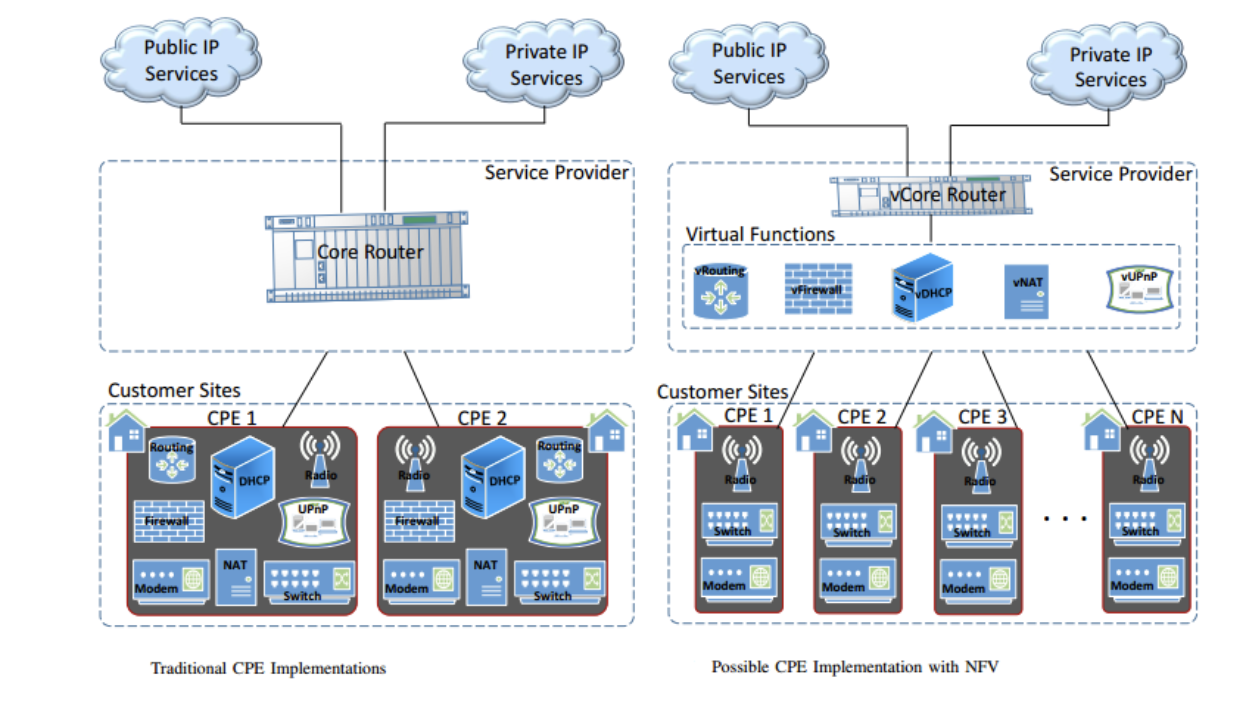
\includegraphics[scale=.5]{images/cpe}
\caption{مجازی‌سازی \lr{CPE}}
\label{fig.20}
\end{figure}

به عنوان مثالی دیگر از موارد کاربرد می توان مجازی‌سازی کارکردها در زیرساخت \lr{LTE} را در نظر گرفت.
در شکل \ref{fig.21} شرایط قبل و بعد از مجازی سازی
\lr{P-GW}، \lr{S-GW}، \lr{PCRF} و \lr{MMF}
نمایش داده شده است.
با مجازی‌سازی این کارکردها علاوه بر استفاده بهتر از منابع، می توان تعداد نمونه‌های آن ها را مطابق با تعداد کاربران بدون تغییر در زیرساخت افزایش و یا کاهش داد.

\begin{figure}[h!]
\center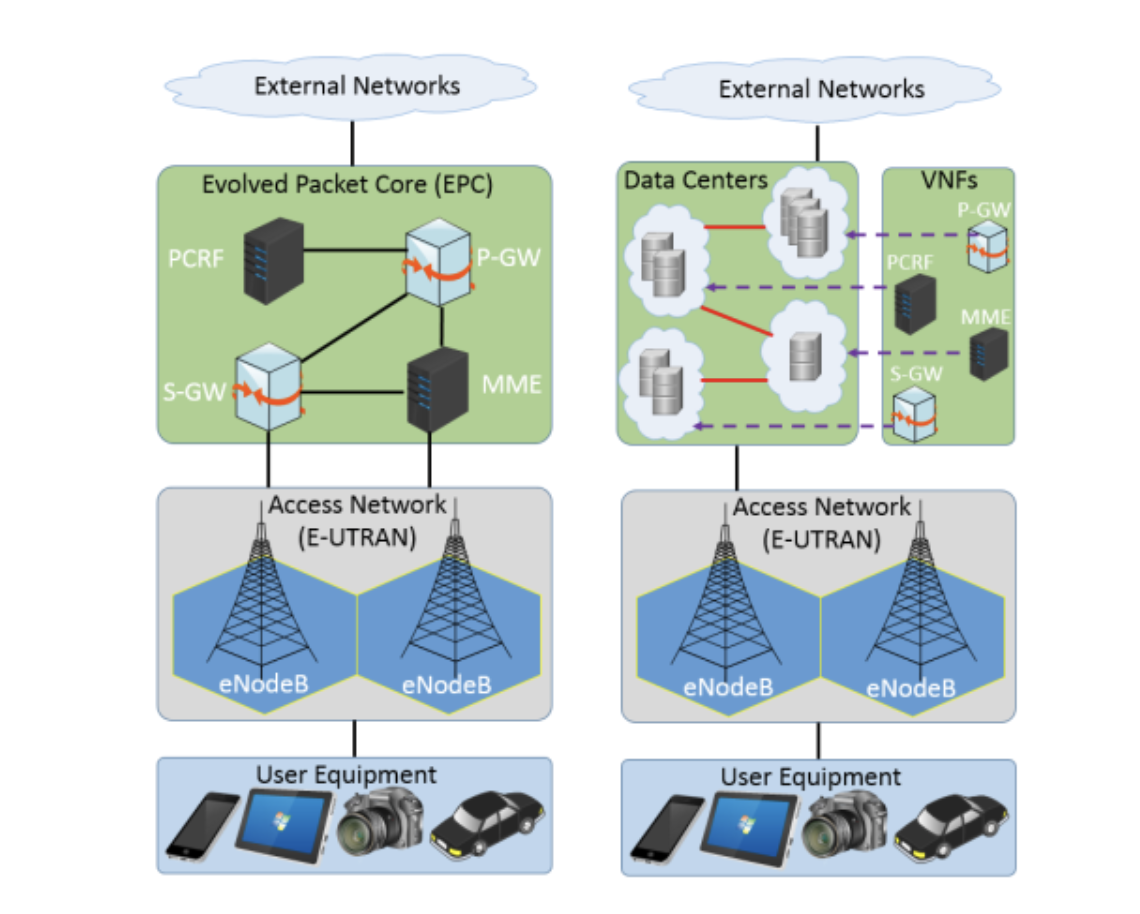
\includegraphics[scale=.5]{images/lte}
\caption{مجازی سازی زیرساخت \lr{LTE}}
\label{fig.21}
\end{figure}

\section{زنجیره‌سازی کارکرد سرویس}

زنجیره سازی کارکردها ایده جدیدی نیست.
در حال حاضر اپراتورها برای ارائه سرویس یک زنجیره از کارکردها ایجاد میکنند که ترافیک کاربر باید از کارکردها با یک ترتیب مشخص عبور کند.
اگرچه همانطور که بیان شد در صورت تغییر در ترتیب کارکردها و یا زنجیره‌ها و یا ایجاد سرویس‌های جدید، نیازمند تغییر مکان فیزیکی کارکردها خواهیم بود
که کاری سخت است و خالی از اشکال نیست.
معماری زنجیره سازی کارکردهای سرویس، اپراتورهای شبکه را قادر می سازد که سرویس های جدید را به صورت نرم افزاری و پویا و بدون اینکه در سطح سخت افزار تغییری ایجاد کنند، ارائه کنند.
در این راستا \lr{IETF} در اسناد متعددی به شرح معماری و اجزای آن پرداخته است.
در این بخش به شرح معماری زنجیره سازی کارکرد سرویس می‌پردازیم و بخش های اصلی آن را بیان می‌کنیم.

\subsection{اجزای معماری \lr{SFC}}

معماری \lr{SFC} توسط \lr{RFC 7665} تعریف شده است.
در این \lr{RFC} یک سرویس شبکه به صورت پیشنهادی که توسط اپراتور ارائه می شود و
از طریق یک یا چند کارکرد سرویس تحویل می‌شود،
تعریف شده است.
یک کارکرد سرویس، رفتار خاصی (به غیر از جلورانی) با بسته را انجام می‌دهد و
و می‌تواند در هر یک از لایه های مدل OSI فعالیت کند.
به یک شبکه یا بخشی از آن که در آن \lr{SFC}  پیاده‌سازی شده است یک دامنه \lr{SFC} گفته می‌شود.
در یک دامنه \lr{SFC}، معماری \lr{SFC} مطابق با شکل \ref{fig.22} پیاده‌سازی می‌شود.

\begin{figure}[h!]
\center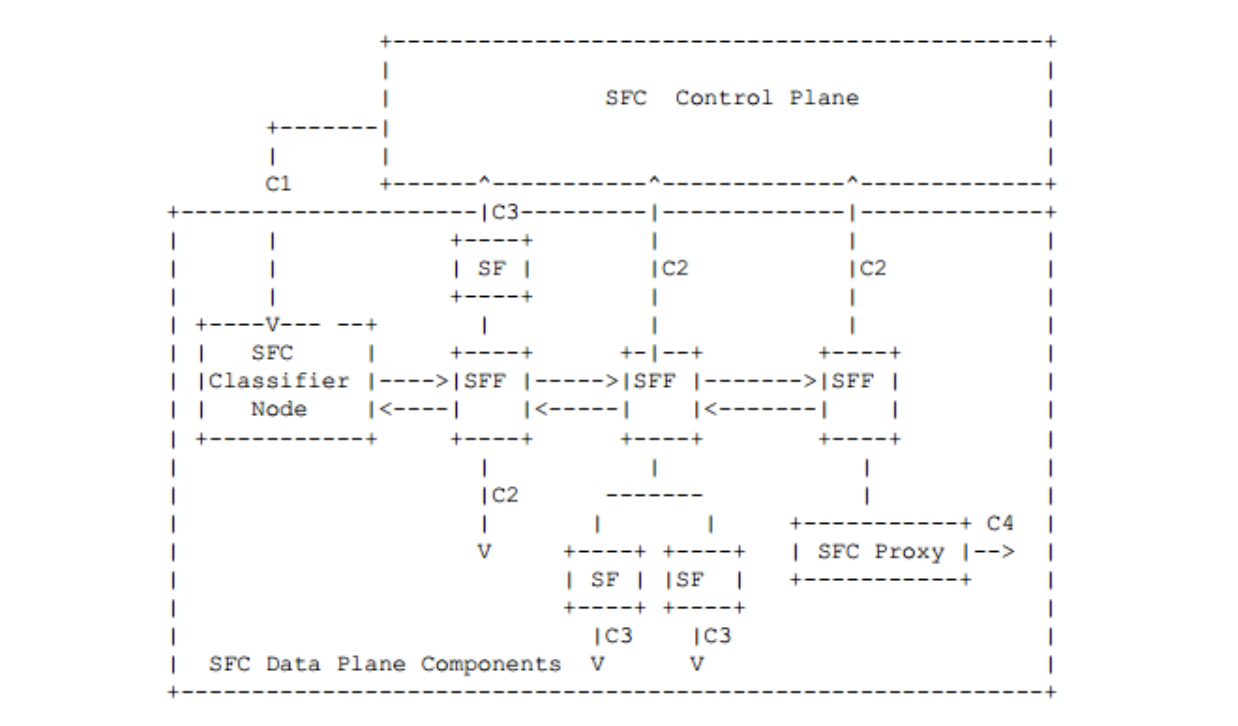
\includegraphics[scale=.5]{images/sfc}
\caption{معماری \lr{SFC}}
\label{fig.22}
\end{figure}